% https://tex.stackexchange.com/a/403931/173708
\documentclass[border=15pt]{standalone}
%\usepackage{showframe}
\usepackage{tikz}
\usetikzlibrary{arrows.meta,positioning}
\usepackage[latin1]{inputenc}

\tikzset{
  line/.style={>=Stealth, semithick, draw=blue!75},
  post/.style={line,->, shorten >=1pt},
  node_box/.style={rectangle, thick, draw=blue!75, fill=blue!10,minimum width=20mm, minimum height=5mm},
  labelnode/.style={auto, sloped, font=\footnotesize,align=center},
}

\begin{document}
%\begin{center}
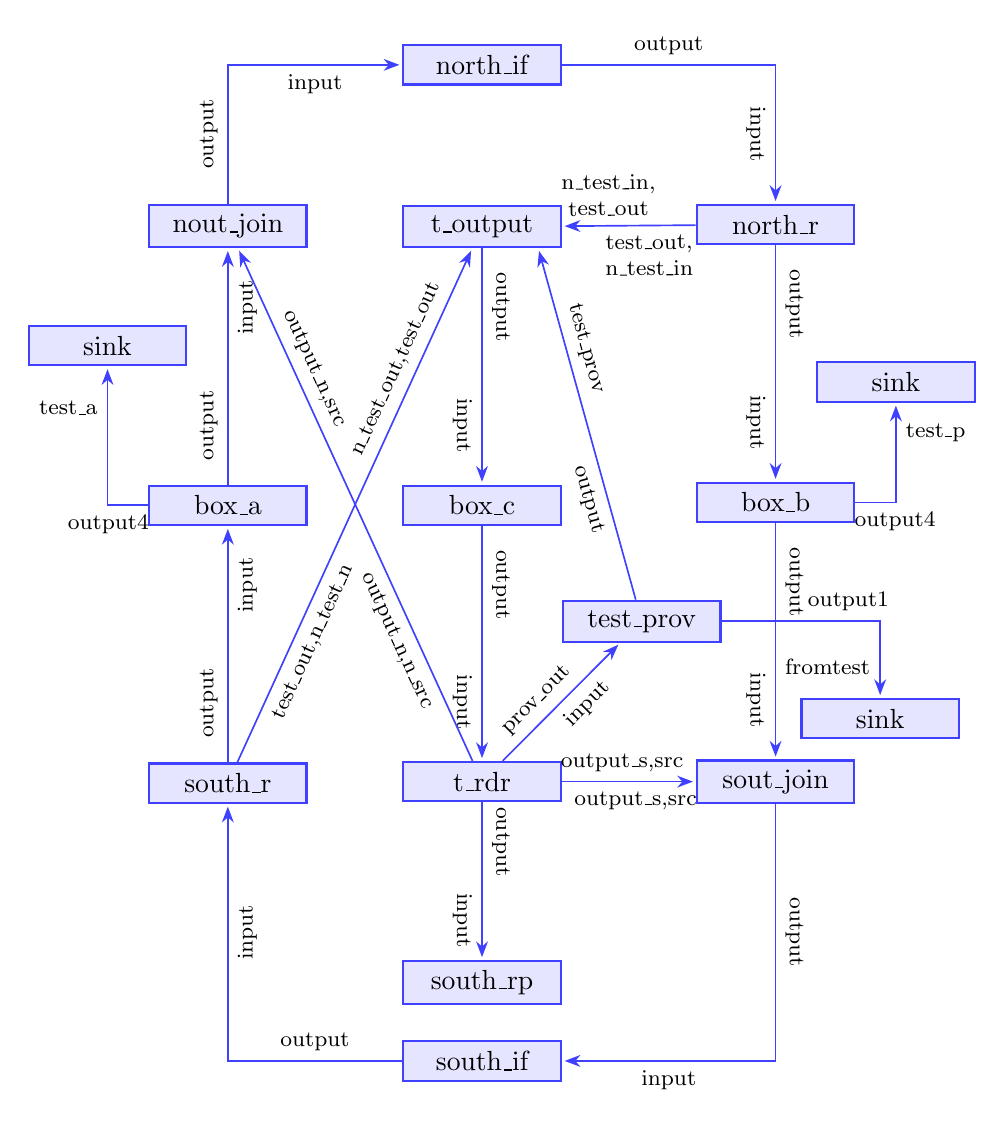
\begin{tikzpicture}[node distance=3cm and 1.7cm]
	\begin{scope}[every node/.style={node_box}]
	  \node                                       (south_if)    {south\_if};
	  \node [above left=of south_if,xshift=5mm]   (south_r)     {south\_r};
	  \node [above=of south_r]                    (box_a)       {box\_a};
	  \node [above=of box_a]                      (nout_join)   {nout\_join};
	  \node [above right=of south_if]             (sout_join)   {sout\_join};
	  \node [above=of sout_join]                  (box_b)       {box\_b};
	  \node [above=of box_b]                      (north_r)     {north\_r};
	  \node [above left=of north_r,yshift=-1.5cm] (north_if)    {north\_if};
	%
	  \node [at={(south_if |- box_a)}]            (box_c)  {box\_c};
	  \node [at={(box_c|-sout_join)}]             (t_rdr)       {t\_rdr};
	%
	  \node [above=of box_c]                       (t_output)    {t\_output};
	  \node [below=2cm of t_rdr]                   (south_rp)    {south\_rp};
	  \node [above right=1.5cm and 0mm of t_rdr]   (test_prov)   {test\_prov};
	  \node [below right=7mm and 1cm of test_prov] (sink_prov)   {sink};
	  \node [above left=1.5cm and -5mm of box_a]   (sink_test_a) {sink};
	  \node [above right=1cm and -5mm of box_b]    (sink_test_p) {sink};
	\end{scope}
	
	\begin{scope}[every node/.style={labelnode}]
	
	\foreach \i/\j in  {%
	    box_b/sout_join,
	    box_a/nout_join,
	    north_r/box_b,
	    box_c/t_rdr,
	    t_rdr/south_rp,
	    t_output/box_c,
	    south_r/box_a}
	  \draw [post] (\i) -- (\j)
	     node[above,near start] {output}
	     node[below,near end,swap] {input};
	
	\foreach \i/\j in{%
	    nout_join/north_if,
	    sout_join/south_if}
	  \draw [post] (\i) |- (\j)
	    node[above,near start] {output}
	    node[below,near end,swap] {input};
	
	\foreach \i/\j in{%
	    north_if/north_r,
	    south_if/south_r}
	  \draw [post] (\i) -| (\j)
	    node[above,near start] {output}
	    node[below,near end,swap] {input};
	
	\draw [post] (t_rdr) -- (test_prov)
	  node[above,pos=0.4] {prov\_out}
	  node[below,pos=0.6] {input};
	
	\draw [post] (test_prov) -- ([xshift=-3mm]t_output.south east)
	  node[above,pos=0.7] {test\_prov}
	  node[below,pos=0.3] {output};
	
	\draw [post] (t_rdr) -- (sout_join)
	  node[above,pos=0.45] {output\_s,src}
	  node[below,pos=0.55] {output\_s,src};
	
	\draw [post] (test_prov) -| (sink_prov)
	  node[above,pos=0.4] {output1}
	  node[left,sloped=false,pos=0.8] {fromtest};
	
	\draw [post] (north_r) -- (t_output)
	  node[above,pos=0.65] {n\_test\_in,\\test\_out}
	  node[below,pos=0.35] {test\_out,\\n\_test\_in};
	
	\draw [post] (box_a) -| (sink_test_a)
	  node[left,sloped=false,pos=0.85] {test\_a}
	  node[below,pos=0.49] {output4};
	
	\draw [post] (box_b) -| (sink_test_p)
	  node[right,sloped=false,pos=0.85] {test\_p}
	  node[below,pos=0.49] {output4};
	
	\draw [post] (t_rdr) -- (nout_join)
	  node[below,near start] {output\_n,n\_src}
	  node[above,near end] {output\_n,src};
	
	\draw [post] (south_r) -- (t_output)
	  node[below,near start] {test\_out,n\_test\_n}
	  node[above,near end] {n\_test\_out,test\_out};
	
	\end{scope}

\end{tikzpicture}
%\end{center}
\end{document}